\documentclass[a4paper,10pt]{article}
\usepackage[utf8]{inputenc}
\usepackage{datetime}
\usepackage{listings}
\usepackage{graphicx}
\usepackage{longtable}
\newdate{date}{31}{03}{2017}
\date{\displaydate{date}}

\title{Mid Term Exam\\Marlen Akimaliev\\BIL622-Numerical Analysis II}
%\author{Share\LaTeX}

\begin{document}

\maketitle

\section{Solve the following Cauchy problem:}
\subsection{Description}
$y''+ 1/5\times y'+ 3.125 \times y = 0$\\
$y(0) = 0$\\
$y'(0) = 1$
\subsection{Solution}
Solution for 100 points as a table in the interval of $t$ at $[0; 10]$ with step size $0.1$ is as follows:
\begin{center}
\begin{longtable}{ |c|c|c| } 
 \hline
 $t$ & $y1$ & $y2$\\
\hline
$   0.00000 $ & $   0.00000 $ & $  1.00000$\\
$   0.10000 $ & $  0.10000 $ & $  1.00000$\\
$   0.20000 $ & $  0.20000  $ & $ 0.96875$\\
$   0.40000 $ & $  0.38750  $ & $ 0.81348$\\
$   0.50000 $ & $  0.46885 $ & $ 0.69238$\\
$   0.60000 $ & $  0.53809  $ & $ 0.54587$\\
$   0.70000 $ & $  0.59267  $ & $ 0.37772$\\
$   0.80000  $ & $ 0.63044 $ & $  0.19251$\\
$   0.90000 $ & $  0.64969 $ & $ -0.00451$\\
$   1.00000 $ & $  0.64924 $ & $ -0.20754$\\
$   1.10000 $ & $  0.62849 $ & $ -0.41043$\\
$  1.20000 $ & $  0.58745 $ & $ -0.60683$\\
$   1.30000  $ & $ 0.52676 $ & $ -0.79041$\\
$   1.40000 $ & $  0.44772 $ & $ -0.95502$\\
$   1.50000 $ & $  0.35222 $ & $ -1.09493$\\
$   1.60000 $ & $  0.24273 $ & $ -1.20500$\\
$   1.70000  $ & $ 0.12223 $ & $ -1.28086$\\
$   1.80000 $ & $ -0.00586  $ & $-1.31905$\\
$   1.90000 $ & $ -0.13776 $ & $ -1.31722$\\
$   2.00000 $ & $ -0.26949 $ & $ -1.27417$\\
$   2.10000 $ & $ -0.39690 $ & $ -1.18996$\\
$  2.20000 $ & $ -0.51590 $ & $ -1.06593$\\
$   2.30000 $ & $ -0.62249 $ & $ -0.90471$\\
$   2.40000 $ & $ -0.71296  $ & $-0.71018$\\
$   2.50000 $ & $ -0.78398 $ & $ -0.48738$\\
$   2.60000 $ & $ -0.83272  $ & $-0.24238$\\
$   2.70000 $ & $ -0.85696 $ & $  0.01784$\\
$   2.80000 $ & $ -0.85517 $ & $  0.28564$\\
$   2.90000 $ & $ -0.82661 $ & $  0.55288$\\
$   3.00000 $ & $ -0.77132 $ & $  0.81119$\\
$   3.10000 $ & $ -0.69020 $ & $  1.05223$\\
$   3.20000 $ & $ -0.58498 $ & $  1.26792$\\
$   3.30000 $ & $ -0.45819 $ & $  1.45072$\\
$   3.40000 $ & $ -0.31311 $ & $  1.59391$\\
$   3.50000 $ & $ -0.15372 $ & $  1.69176$\\
$   3.60000 $ & $  0.01545 $ & $  1.73979$\\
$   3.70000 $ & $  0.18943 $ & $  1.73496$\\
$   3.80000 $ & $  0.36293 $ & $  1.67577$\\
$   3.90000  $ & $ 0.53051 $ & $  1.56235$\\
$   4.00000  $ & $ 0.68674 $ & $  1.39657$\\
$   4.10000 $ & $  0.82640  $ & $ 1.18196$\\
$   4.20000 $ & $  0.94459 $ & $  0.92371$\\
$   4.30000$ & $   1.03697$ & $   0.62853$\\
$   4.40000  $ & $ 1.09982  $ & $ 0.30448$\\
$   4.50000  $ & $ 1.13027 $ & $ -0.03922$\\
$   4.60000 $ & $  1.12634$ & $  -0.39243$\\
$   4.70000  $ & $ 1.08710  $ & $-0.74441$\\
$   4.80000 $ & $  1.01266 $ & $ -1.08413$\\
$   4.90000 $ & $  0.90425 $ & $ -1.40058$\\
$   5.00000  $ & $ 0.76419$ & $  -1.68316$\\
$   5.10000 $ & $  0.59587 $ & $ -1.92197$\\
$   5.20000 $ & $  0.40368 $ & $ -2.10818$\\
$   5.30000 $ & $  0.19286 $ & $ -2.23433$\\
$   5.40000  $ & $-0.03057 $ & $ -2.29460$\\
$   5.50000 $ & $ -0.26003 $ & $ -2.28504$\\
$   5.60000 $ & $ -0.48854 $ & $ -2.20378$\\
$   5.70000  $ & $-0.70892 $ & $ -2.05111$\\
$   5.80000 $ & $ -0.91403 $ & $ -1.82958$\\
$   5.90000 $ & $ -1.09699 $ & $ -1.54394$\\
$   6.00000  $ & $-1.25138 $ & $ -1.20114$\\
$   6.10000 $ & $ -1.37149 $ & $ -0.81008$\\
$   6.20000 $ & $ -1.45250 $ & $ -0.38149$\\
$   6.30000 $ & $ -1.49065 $ & $  0.07242$\\
$   6.40000  $ & $-1.48341  $ & $ 0.53825$\\
$   6.50000 $ & $ -1.42958  $ & $ 1.00181$\\
$   6.60000 $ & $ -1.32940  $ & $ 1.44856$\\
$   6.70000 $ & $ -1.18455 $ & $  1.86400$\\
$   6.80000 $ & $ -0.99815  $ & $ 2.23417$\\
$   6.90000  $ & $-0.77473  $ & $2.54609$\\
$   7.00000 $ & $ -0.52012  $ & $ 2.78819$\\
$   7.10000  $ & $-0.24130 $ & $  2.95073$\\
$   7.20000 $ & $  0.05377  $ & $ 3.02614$\\
$   7.30000 $ & $  0.35638  $ & $ 3.00933$\\
$   7.40000 $ & $  0.65732  $ & $ 2.89796$\\
$   7.50000  $ & $ 0.94711 $ & $  2.69255$\\
$   7.60000 $ & $  1.21637 $ & $  2.39658$\\
$   7.70000 $ & $  1.45603 $ & $  2.01646$\\
$   7.80000$ & $   1.65767$ & $   1.56145$\\
$   7.90000 $ & $  1.81382 $ & $  1.04343$\\
$   8.00000 $ & $  1.91816 $ & $  0.47661$\\
$   8.10000  $ & $ 1.96582 $ & $ -0.12281$\\
$   8.20000 $ & $  1.95354 $ & $ -0.73713$\\
$   8.30000 $ & $  1.87983 $ & $ -1.34761$\\
$   8.40000 $ & $  1.74507 $ & $ -1.93506$\\
$   8.50000  $ & $ 1.55156 $ & $ -2.48039$\\
$   8.60000$ & $   1.30352$ & $  -2.96526$\\
$   8.70000  $ & $ 1.00700 $ & $ -3.37261$\\
$   8.80000  $ & $ 0.66974 $ & $ -3.68729$\\
$   8.90000  $ & $ 0.30101 $ & $ -3.89659$\\
$   9.00000 $ & $ -0.08865$ & $  -3.99065$\\
$   9.10000$ & $  -0.48772$ & $  -3.96295$\\
$   9.20000  $ & $-0.88401$ & $ -3.81053$\\
$   9.30000  $ & $-1.26507 $ & $ -3.53428$\\
$   9.40000  $ & $-1.61849 $ & $ -3.13895$\\
$   9.50000 $ & $ -1.93239 $ & $ -2.63317$\\
$   9.60000 $ & $ -2.19571 $ & $ -2.02930$\\
$   9.70000 $ & $ -2.39863 $ & $ -1.34314$\\
$   9.80000 $ & $ -2.53295 $ & $ -0.59357$\\
$   9.90000 $ & $ -2.59231$ & $   0.19798$\\
$  10.00000  $ & $-2.57251 $ & $  1.00808$\\
 \hline
\end{longtable}
\end{center}
I have used the following Python code \cite{inp} to evaluate values and plot the graph.
\begin{lstlisting}[language=Python]
#  Solves a Cauchy problem for a 2nd order ODE by Euler's method
#		y" + 1/5y'+3.125y = 0, y(0) = 0, y'(0) = 1
#  Equivalent problem: y[1] = y, y[2] = y'
#     y[1]' =  y[2],   y[1](0) = 0
#     y[2]' = -3.125y[1]-1/5y[2],   y[2](0) = 1
#----------------------------------------------------------------------------
from math import *
from ode import *
from matplotlib import pyplot as plt

def Func(t, y, f):                                 # Right-hand sides of ODEs
	f[1] =  y[2]
	f[2] = -3.125*y[1]-1/5*y[2]

# main

y0 = 0; dy0 = 1                         # initial values => y(t) = sin(t)
tmax = 10e0                                                      # time span
ht = 0.1e0                                                       # step size

n = 2                                              # number of 1st order ODEs
nt = int(tmax/ht + 0.5) + 1                            # number of time steps
y = [0]*(n+1)                                           # solution components

out = open("ode.txt","w")                                  # open output file
out.write("      t         y1        y2\n")

t = 0e0
y_1 = []
y_2 = []

y[1] = y0; y[2] = dy0                                        # initial values
out.write(("{0:10.5f}{1:10.5f}{2:10.5f}\n"). \
          format(t,y[1],y[2]))

y_1.append(y[1])
y_2.append(y[2])

while (t+ht <= tmax):                                      # propagation loop
   Euler(t,ht,y,n,Func)
   t += ht
	
   y_1.append(y[1])
   y_2.append(y[2])

   out.write(("{0:10.5f}{1:10.5f}{2:10.5f}\n"). \
             format(t,y[1],y[2]))
out.close()

plt.plot(y_1, y_2)
plt.title( "Euler method")
plt.xlabel('Value of y[1]') 
plt.ylabel('Value of y[2]')
plt.legend(loc=4)
plt.grid()
plt.savefig( '1_1.eps', fmt='EPS', dpi=100 )
plt.show()
\end{lstlisting}
Plot for these values will be as follows:
\begin{figure}[ht]
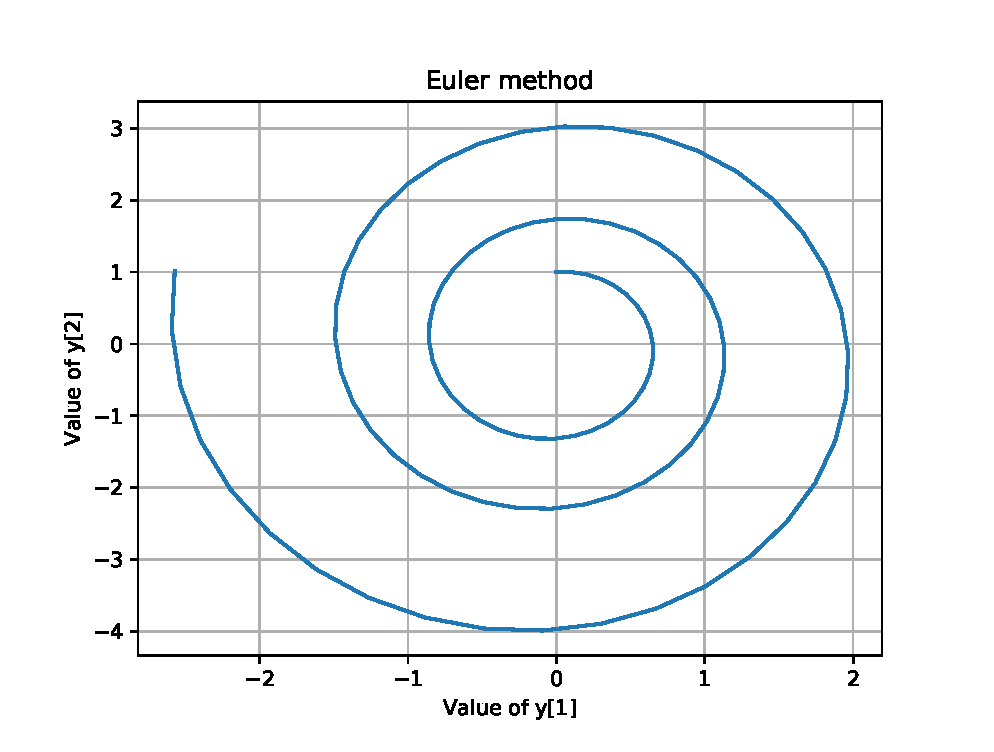
\includegraphics[width=8cm]{1_1.eps}
\end{figure}

\section{Solve the following Boundary Value Problem:}
\subsection{Description}
$y''+ (x-1)\times y'+ 3.125 \times y = 4\times x$\\
$y(0) = 1$\\
$y(1) = 1.368$
\subsection{Solution}
I have used the following Python code \cite{bvp} to evaluate values and plot the graph.
\begin{lstlisting}[language=Python]
#	$y''+ (x-1)y'+ 3.125y = 4x$\\
#	y(0) = 1
#	y(1) = 1.368
#	y1' = y2
#	y2' = 4x-(x-1)y2 - 3.125y1

import numpy as np
from scipy.integrate import solve_bvp
import matplotlib.pyplot as plt

def fun(x, y, p):
	x = p[0]
	return np.vstack((y[1], 4*x-(x-1)*y[1] - 3.125*y[0]))

def bc(ya, yb, p):
	k = p[0]
	return np.array([ya[0], yb[0], ya[1] - k])

x = np.linspace(0, 1, 5)
y = np.zeros((2, x.size))
y[0, 1] = 1
y[0, 3] = 1.3

sol = solve_bvp(fun, bc, x, y, p=[5])
print sol.p[0]

x_plot = np.linspace(0, 1, 100)
y_plot = sol.sol(x_plot)[0]
plt.plot(x_plot, y_plot)
plt.grid()
plt.xlabel("x")
plt.ylabel("y")
plt.show()
\end{lstlisting}
Plot for these values will be as follows:
\begin{figure}[ht]
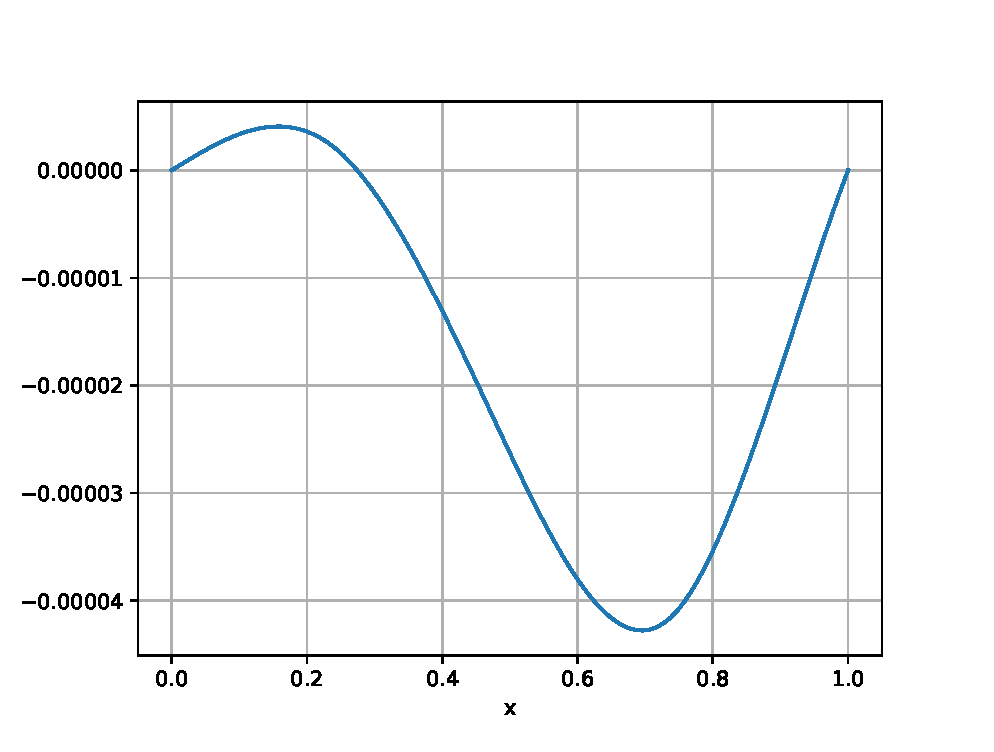
\includegraphics[width=8cm]{1_2.eps}
\end{figure}
\medskip

\begin{thebibliography}{9}
\bibitem{inp} Introduction to Numerical Programming, \\\texttt{http://phys.ubbcluj.ro/~tbeu/INP/programs.html}
\bibitem{bvp} scipy.integrate.solve-bvp, \\\texttt{https://docs.scipy.org/doc/scipy-0.18.1/reference/generated/scipy.integrate.solve-bvp.html}

\end{thebibliography}

\end{document}
